\documentclass[smaller]{beamer}
\usepackage{beamerarticle}
\mode<presentation> {
  \usetheme{Montpellier}
  \useinnertheme{circles}
  \usecolortheme{sidebartab}
  \setbeamercolor{structure}{fg=blue}
  % or ...

%  \setbeamercovered{transparent}
  % or whatever (possibly just delete it)
}
\usepackage{movie15}
\usepackage[utf8]{inputenc}

\usepackage[english,russian]{babel}
\usepackage{listings}
\usepackage[T2A]{fontenc}
%\usepackage{amssymb,amsmath,mathrsfs,amsthm}

\usepackage[footnotesize]{caption2}
\usepackage{indentfirst}
\usepackage{multicol}
%\usepackage[cp1251]{inputenc}
% %\usepackage[russian]{babel}
\usepackage{amssymb,amsmath}

%\usepackage[T2A]{fontenc}
\usepackage[utf8]{inputenc}
\usepackage{graphicx, graphics, epsfig}
\usepackage{epstopdf}
\usepackage{ifpdf}  
%\usepackage[scaled=.92]{helvet}
%\usepackage{times}
\usepackage{mathrsfs}
\usepackage{amsfonts}
\usepackage{floatflt}

%\usepackage[pdftex,unicode]{hyperref}
%\usepackage[cp1251]{inputenc}
%\usepackage[utf8]{inputenc}
%\usepackage{listings}
%\usepackage[pdftex,unicode]{hyperref}
%\usepackage[english]{babel}
%\usefonttheme{serif}
% Or whatever. Note that the encoding and the font should match. If T1
% does not look nice, try deleting the line with the fontenc.


\title{Вероятностный подход к поиску поведенческих
паттернов} % (optional, use only with long paper titles)

\author % (optional, use only with lots of authors)
[~]{Вишневский В.В.}


\AtBeginSubsection[] {
  \begin{frame}<beamer>
    \frametitle{Plan}
    \tableofcontents[currentsection,currentsubsection]
  \end{frame}
}
\begin{document}

\begin{frame}
  \titlepage
\end{frame}

%\begin{frame}
 % \frametitle{План}
 % \tableofcontents
  % You might wish to add the option [pausesections]
%\end{frame}



\section{Исследование поведения}


\begin{frame}	
 \frametitle{Входные данные}

%\begin{figure}[ht]
%\includemovie[poster,text={\includegraphics[width=8cm, height=6cm]
%{beh_data.eps}},autoplay,mouse=true]{8cm}{6cm}
%{video_kth.avi}
%\end{figure}
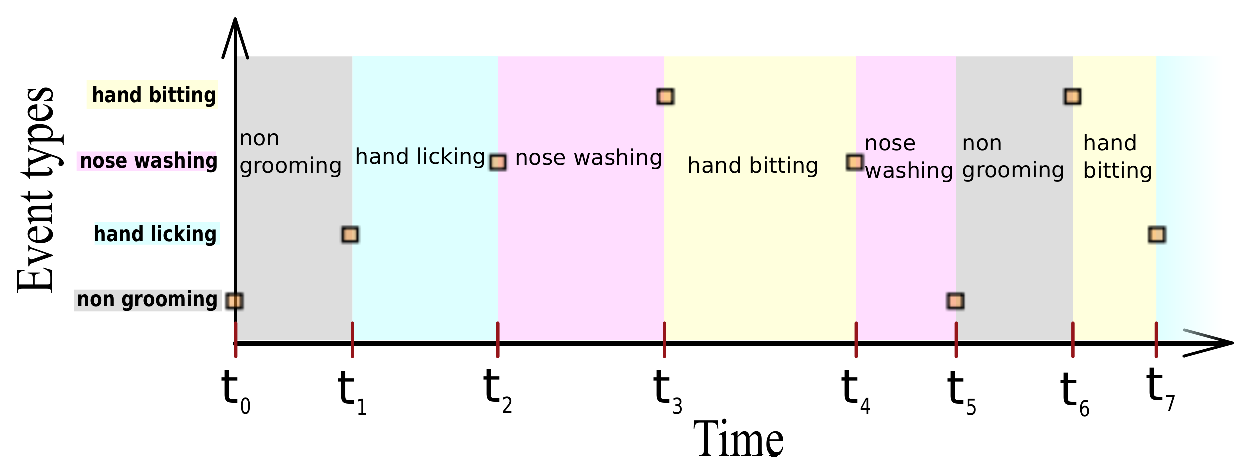
\includegraphics[scale=0.5]{beh_data.eps}
%\begin{figure}[ht]
%\includemovie[
%poster,
%label=cells,
%  text={\small Test mplayer with acroread}
  %mimetype=video/mpg,
%]{12cm}{6cm}{video_kth.avi}
%\end{figure}

  %  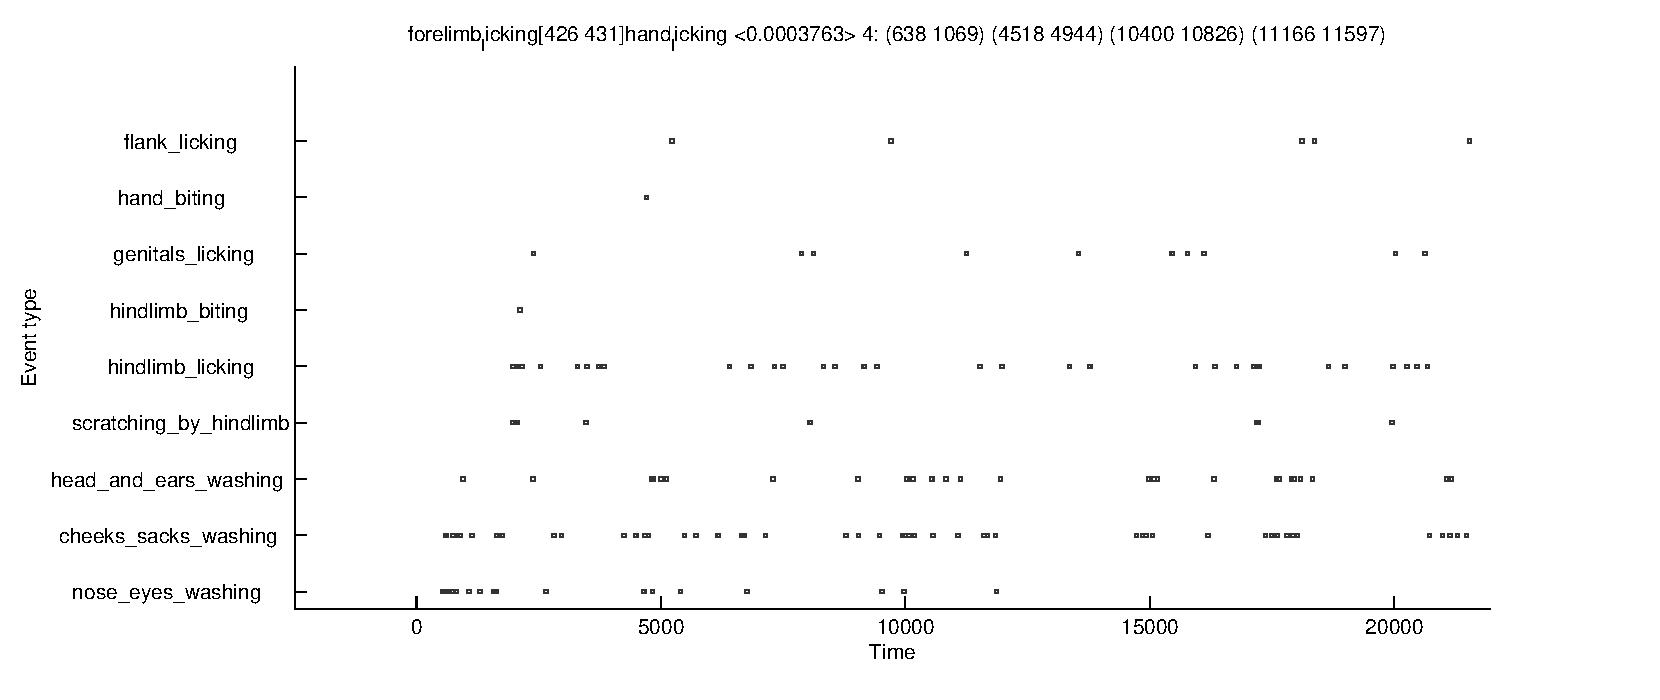
\includegraphics[scale=0.4]{TS.eps} 
\end{frame}


\begin{frame}	
  \frametitle{Подход к поиску паттернов}
Паттерн~--- это часто встречающаяся последовательность событий(поведенческих актов), возникающих один за другим 
через определенные промежутки времени.
\\~\\
  Инициализируем множество паттернов поведенческими актами. Потом итеративно повторяем:
  \begin{itemize}
   \item {\bf Конструирование:}Для всех пар паттернов проверить, повторяется ли один за другим достаточно часто. Если да, 
	то получаем новый паттерн. 
   \item {\bf Редукция:} Удалить одинаковые паттерны, которые были сконструированы по-разному.
  \end{itemize}
\end{frame}

\section{Т-Паттерны}
\begin{frame}	
  \frametitle{Понятие Т-Паттерна(M.S. Magnusson)}
  \begin{itemize}
   \item События соединеятся критическими интервалами. $A[dA_l,dA_r]B[dB_l,dB_r]C\dots F$. 
   \item Критический интервал ($A[d_1,d_2]B$) -- это связь между двумя паттернами, означающая, что паттерн $B$ появляется 
в промежутке $[d_1,d_2]$ 
после паттерна $A$ \emph{чаще, чем ожидается}.
\\ 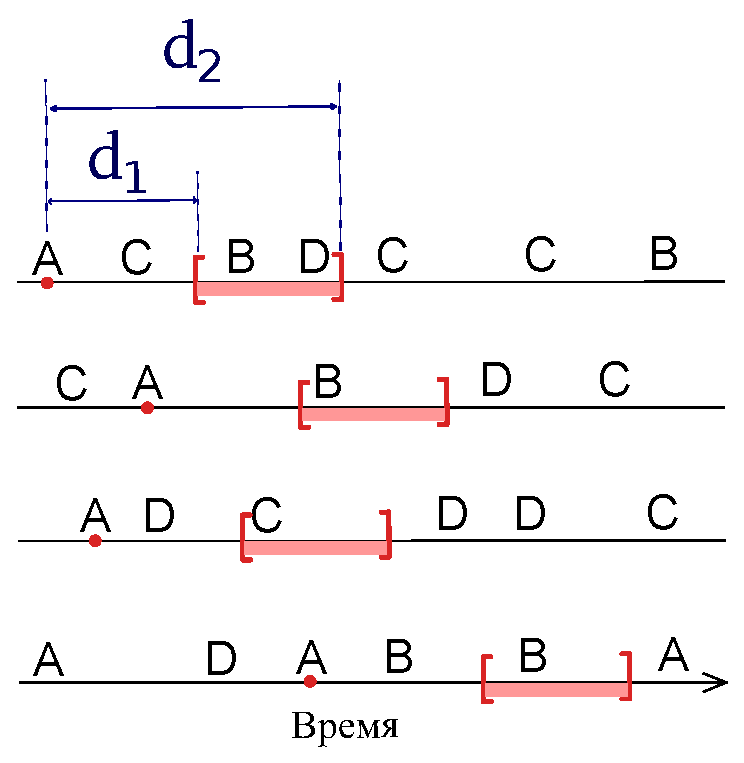
\includegraphics[scale=0.30]{TPTSn.eps} 
  \end{itemize}
\end{frame}

\begin{frame}	
  \frametitle{чаще, чем ожидается}
\begin{itemize}
   \item Гипотеза $H_0$: события распределены равномерно и независимо. То есть закономерностей нету.
   \item Считаем вероятность входных данных при условии $H_0$.
   \item Если эта вероятность мала(меньше $\alpha$) $\Longrightarrow$ мы отвергаем $H_0$ и считаем, что существует закономерность.
\end{itemize}
\end{frame}

\begin{frame}	
  \frametitle{Типы <<лишних>> паттернов}
\begin{itemize}
 \item {\bf Дубликаты:} $(AB)(CD)$ и $(A(BC))D$
  \\ 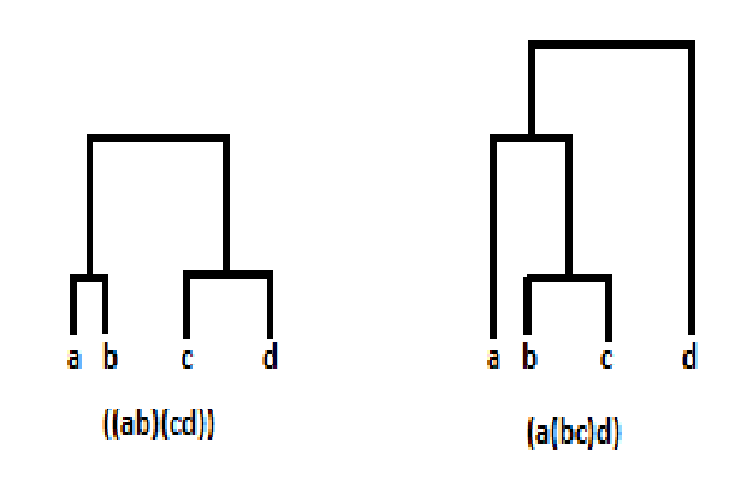
\includegraphics[scale=0.37]{dup_tree.eps} 
 \item {\bf Неполные копии:} $(BCD)$ не встречается вне $(ABCD)$
  \\ 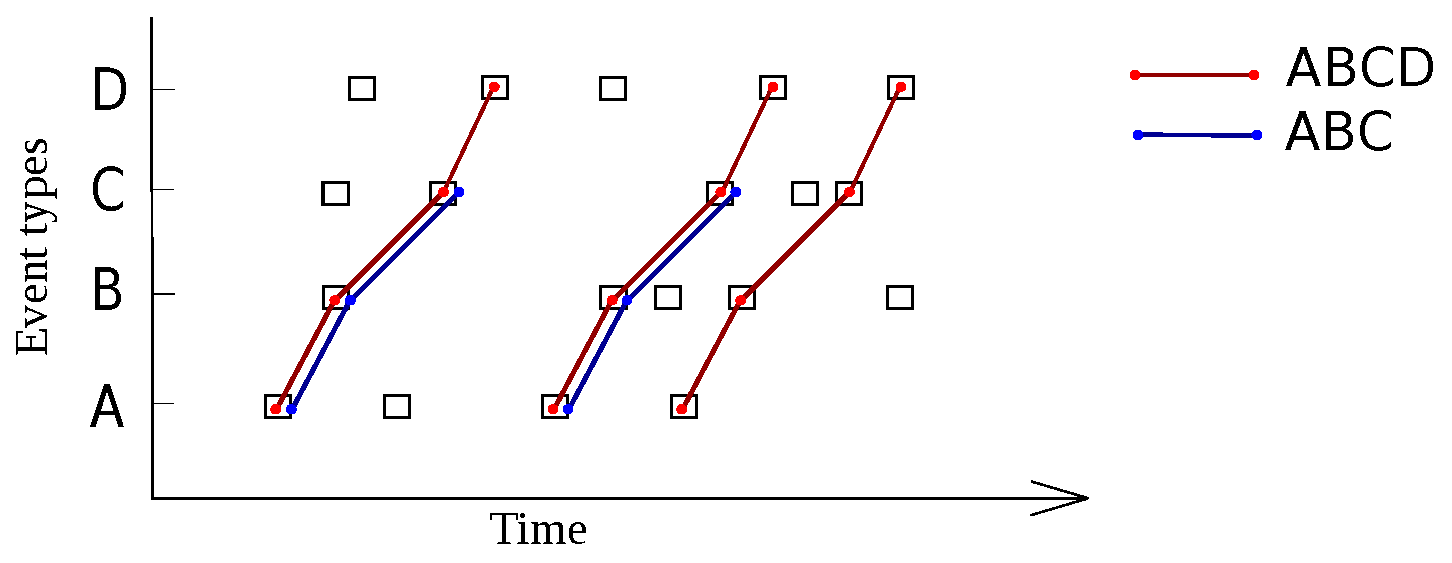
\includegraphics[scale=0.30]{dup_2.eps} 
\end{itemize}
\end{frame}

\begin{frame}
  \frametitle{Недостатки Т-Паттернов}
  \begin{itemize}
   \item Чувствительность к шуму и пропускам в исходных данных.
   \item Часто выделяется слишком много похожих паттернов.
   \item Закрытые исходные коды.
  \end{itemize}
\end{frame}




\section{P-Паттерны}
\begin{frame}
\frametitle{Вероятностная модель P-Паттерна}
 \begin{itemize}
  \item $P=A[\mu_A,\sigma_A]B[\mu_B,\sigma_B]C[\mu_C,\sigma_C]$\\
 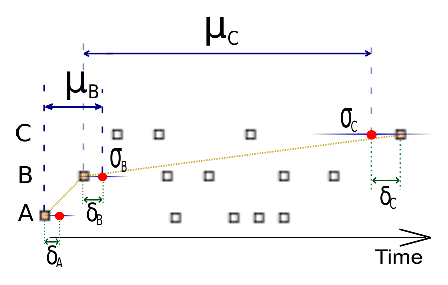
\includegraphics[scale=0.6]{il1.eps} \\
  \item Функция потерь:
        $$
  f_{LOSS}(x,N)= \begin{cases}
   \exp\bigl(-\frac{\lambda x}{N}\bigr), & x < N, \\
   0,                                    & x=N.
   \end{cases}
  $$
  \item Правдоподобие паттерна:
$$L_{P}(\varepsilon)=
f_{LOSS}(N_-,N_{P})
\prod_{i=1}^{N_{P}}\left( \frac1{\sqrt{2\pi}\,\sigma_i }\right) 
\prod_{i\in \mathcal{N}_+}\exp\left(- \frac{\delta_i^2}{2\sigma_i^2}\right) 
$$
 \end{itemize}
\end{frame}  

\begin{frame}
\frametitle{Правдоподобие}
\begin{figure}[H]
\noindent\centering{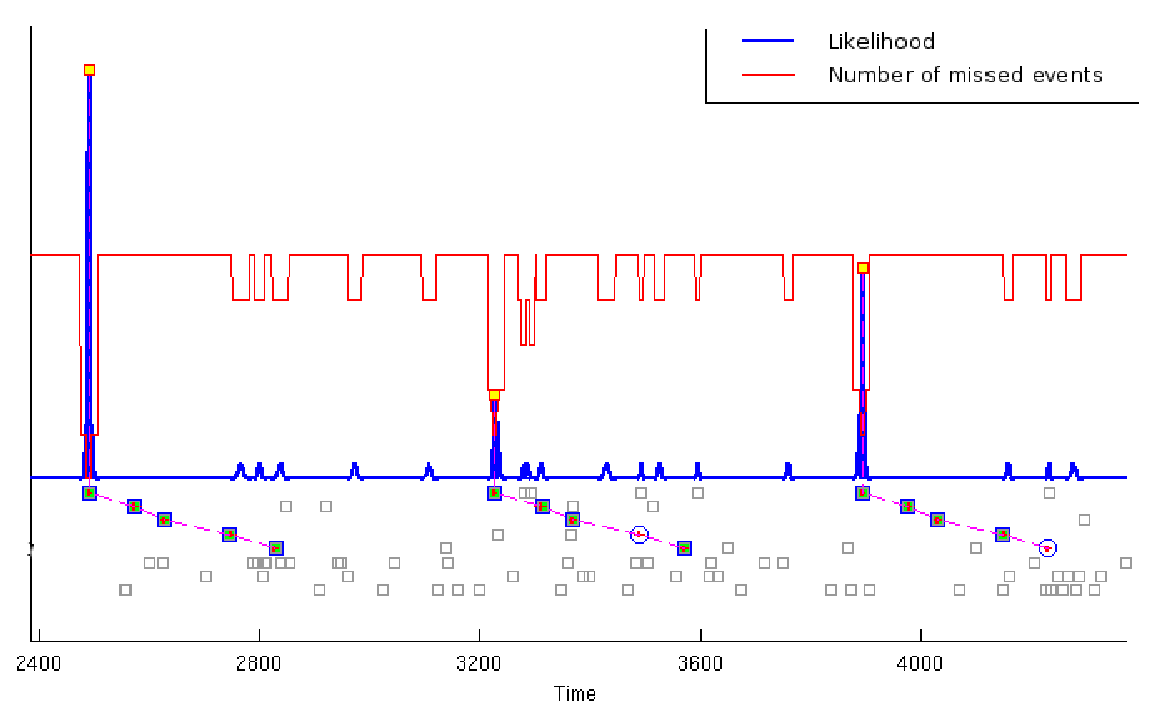
\includegraphics[scale=0.4]{norm_12_of_14.eps}}
\caption{ Пример функции правдоподобия паттерна. Желтыми маркерами с красной границей изображены максимумы функции правдоподобия: 
моменты времени, когда мы считаем, что паттерн имеет место.
В нижней части рисунка закрашенными квадратами показаны присутствующие
события, полыми кружками~--- пропущенные события в паттерне. Полые серые квадраты соответствуют наблюдаемым поведенческим актам.}
\end{figure}
\end{frame}  

\begin{frame}
\frametitle{Конструирование новых паттернов}
\begin{itemize}
 \item Вводится модель связи событий:
$$g_{\mu,\sigma}(x_i)=\frac{1}{\sqrt{2\pi}\,\sigma}\exp\left(- \frac{(x_i-\mu)^2}{2\sigma^2} \right).$$
\item Тестируется против гипотезы о равномерном, случайном, независимом распределении событий.
\item Долгий перебор по $\mu$ и $\sigma$.
\end{itemize}
\end{frame}  

\begin{frame}
\frametitle{Удаление паттернов}
Корреляция векторов значений функции правдоподобия:
$$
cor\left(\overrightarrow{L_1}, \overrightarrow{L_2}\right) = 
\frac{{\overrightarrow{L_1}}^\top \overrightarrow{L_2}}{ 
\sqrt{ {\overrightarrow{L_1}}^\top \overrightarrow{L_1} }\,\sqrt{ {\overrightarrow{L_2}}^\top \overrightarrow{L_2} } }
\:\in[\,0,1]
$$
~--- коэффициент корреляции между двумя P-Паттернами. Чем он ближе к $1$, тем два паттерна 
более близки друг к другу.
\end{frame}  

\begin{frame}
  \frametitle{ Параметры предложенного метода }
    {\small
   \begin{tabular}{|p{2em} | p{5em} | p{3em} | p{12em}| }
    \hline
    \bf{Пар-р} & \bf{ Возможные\newline значения} & \bf{ defaults } &\bf{ На что влияет } \\
    \hline\hline
    \centering$\alpha$   & \centering$[\,0, 1]$ & \centering $0.001$ & Уровень значимости паттерна \\ \hline
    \centering$N_{min}$ &  \centering$[\,0, +\infty]$ & \centering 3 & Минимальное количество появлений паттерна в данных  \\ \hline \hline 
    \centering$\lambda$  & \centering$[\,0, +\infty]$ & \centering 8 & Допустимая степень нечеткости паттерна  \\  \hline    
    \centering$\nu$      & \centering$[\,0, 1]$ & \centering 0.6 & Минимальная степень похожести паттернов для удаления \\ \hline
    \centering$\gamma$   & \centering$[\,0, 1]$ & \centering 0.4 & Чувствительность к отклонению от ожидаемого правдоподобия \\ \hline
\end{tabular}}

\end{frame}


\section{Параллельная реализация}
\begin{frame}
  \frametitle{Т-Паттерны и P-Паттерны}
  \begin{itemize}
   \item T-Паттерны распараллеливаем на SMP с помощью OpenMP. Тестирование на 4-х ядерном CPU.
  \item P-Паттерны распараллеливаем на GPU с помощью CUDA. Тестирование на GF 8800GTX, 128 потоковых процессора.
  \end{itemize}
\end{frame}

\begin{frame}
 \frametitle{Ускорение OpenMP}
\begin{figure}[H]
\centering{	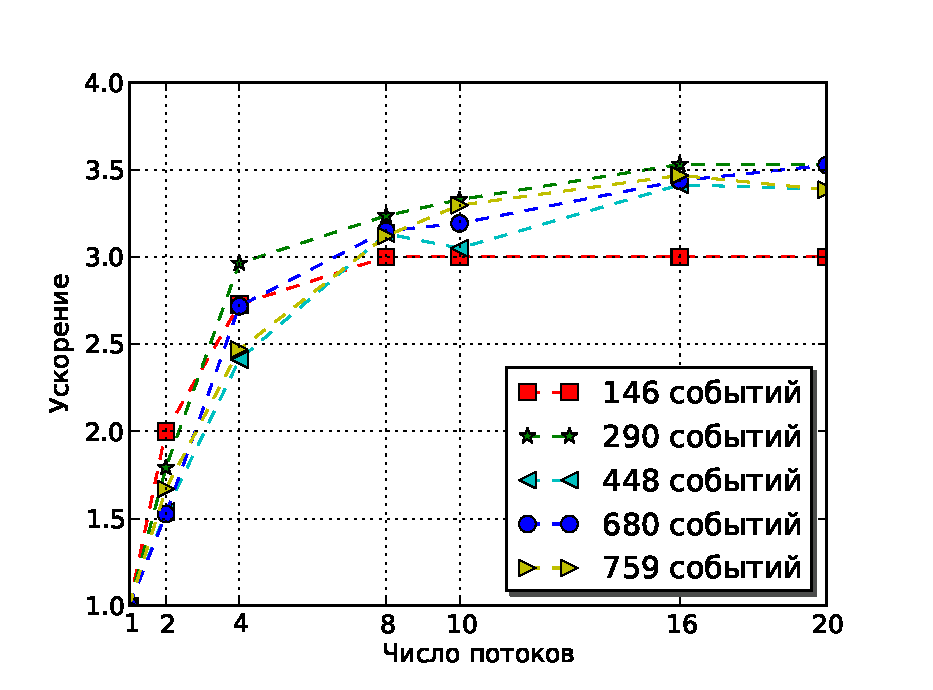
\includegraphics[scale=0.5]{omp_su.eps} }
	\caption{Ускорение алгоритма поиска Т-Паттернов на 4-х ядерном процессоре.}
\end{figure}
    
\end{frame}


\begin{frame}
  \frametitle{Ускорение алгоритма поиска P-Паттернов. CUDA}
\begin{figure}[H]
\centering{	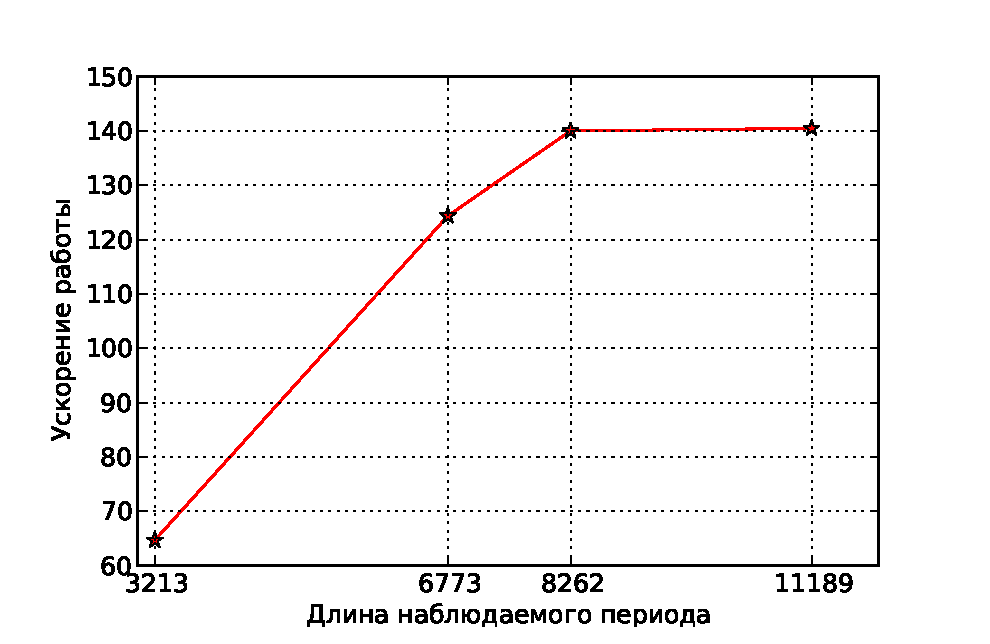
\includegraphics[scale=0.45]{cuL_su.eps} }
	\caption{Ускорение стадии подсчета правдоподобия паттернов в зависимости от размера входных данных.}
\end{figure}

\end{frame}

\begin{frame}
  \frametitle{Ускорение алгоритма поиска P-Паттернов. CUDA}
\begin{figure}[H]
\centering{	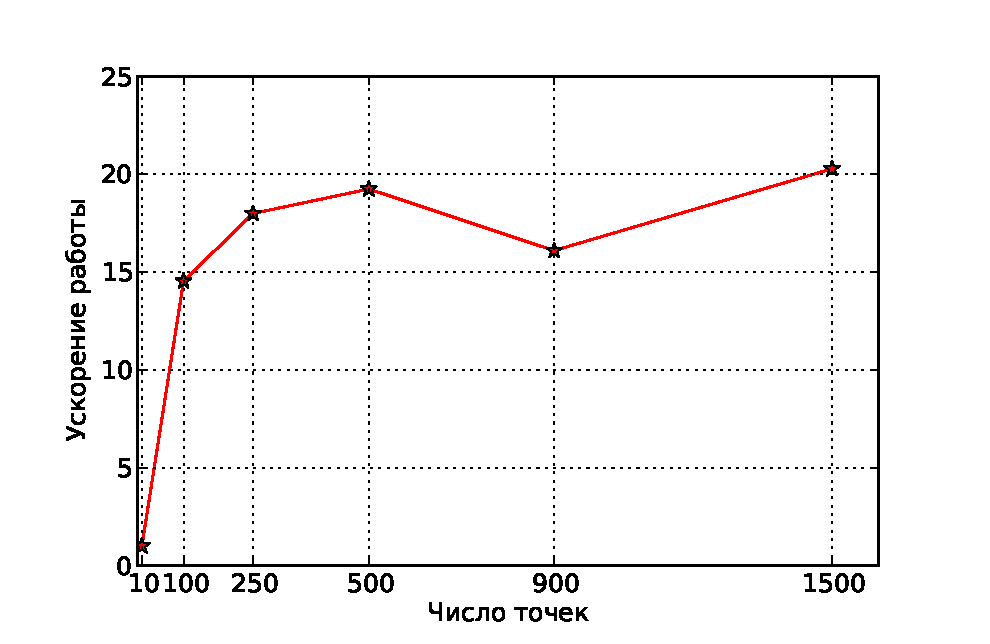
\includegraphics[scale=0.3]{cuD_su.eps} }
	\caption{Ускорение стадии конструирования паттернов в зависимости от размера входных данных.}
\end{figure}

Ускорение метода в целом $\sim$ 40 раз. \\
Типичные экспериментальные данные: 12 секунд на GPU, 470 секунд на CPU(1 поток).\\
Утилизация GPU $\sim$ 230 GFLOPS (Заявленная производительность 518 GFLOPS)

\end{frame}


\section{Эксперимент на реальных данных}

\begin{frame}
  \frametitle{Эксперимент с грызунами без гиппокампа}
  \begin{itemize}
   \item Гиппокамп~--- отдел головного мозга. Его функции 
связывают с механизмами работы памяти, обучением, пространственной
навигацией.
   \item Две группы: контрольная(12 особей) и грызуны без гиппокампа(12 особей).
   \item Определить по поведению к какой группе относится особь.
  \end{itemize}
\begin{figure}[H]
\centering{	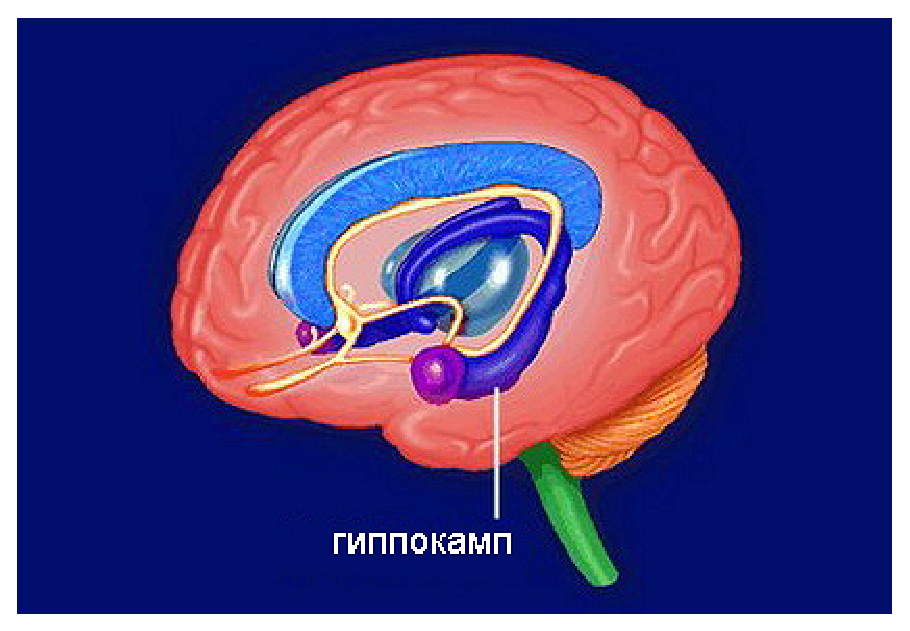
\includegraphics[scale=0.3]{hippocamp.eps} }
\end{figure}
\end{frame}

\begin{frame}
  \frametitle{Результаты экспериментов}
\begin{figure}[H]
\noindent\centering{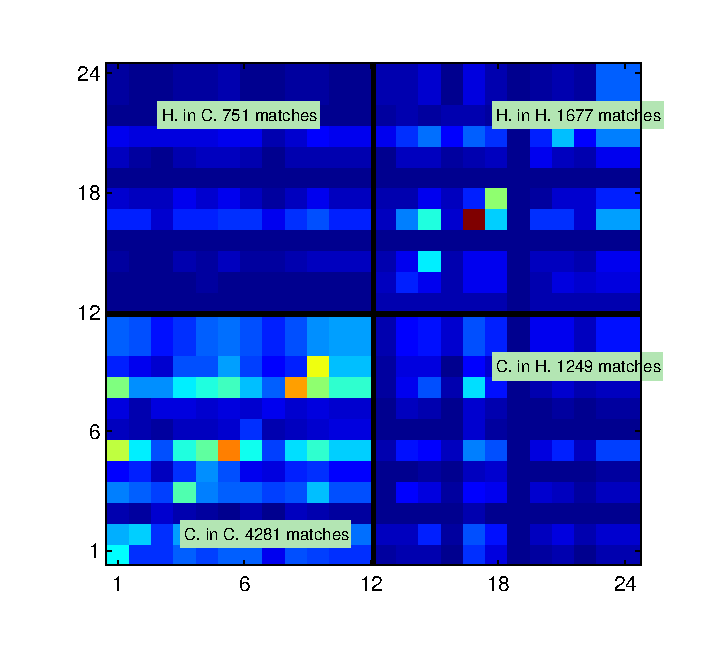
\includegraphics[scale=0.5]{cross_m_big.eps}}
\caption{ Таблица соответствий паттернов. Неформально: 
по вертикали {\em откуда} берутся паттерны, по горизонтали~--- {\em где} ищутся вхождения этих паттернов; например, в ячейке $(3,10)$ записано
число соответствий паттернов третей особи в поведении десятой.}

\end{figure}
\end{frame}

\begin{frame}
  \frametitle{Классификация}
\begin{itemize}
 \item группа 1: контроль,
\item группа 2: гиппокампальная,
\item группа 3: шум с параметрами частоты и длины\\ актов от группы 1,
\item группа 4: шум с параметрами частоты и длины\\ актов от группы 2,
\item группа 5: данные содержащие 1 искусственный паттерн.
\end{itemize}
\end{frame}

\begin{frame}

\begin{figure}[h]
\noindent\centering{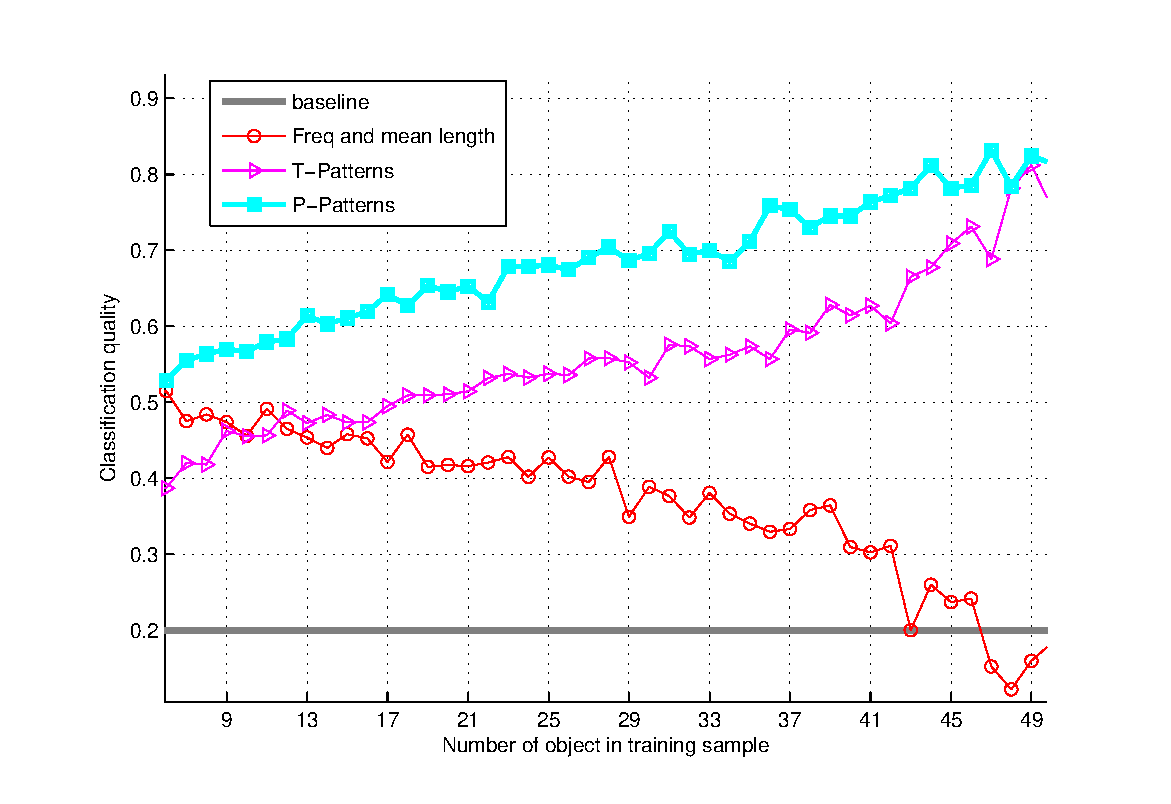
\includegraphics[width=93mm]{bad_data.eps}}
\caption{ Качество~--- средняя доля правильных классификаций.
По горизонтали откладывалось количество объектов в обучении(для каждого значение качество усреднялось по ста повторениям с разными разбиениями для обучения).
 }
\end{figure}
\end{frame}

\begin{frame}
  \frametitle{Классификация}
\begin{figure}[H]
	\begin{multicols}{2}
	\hfill
	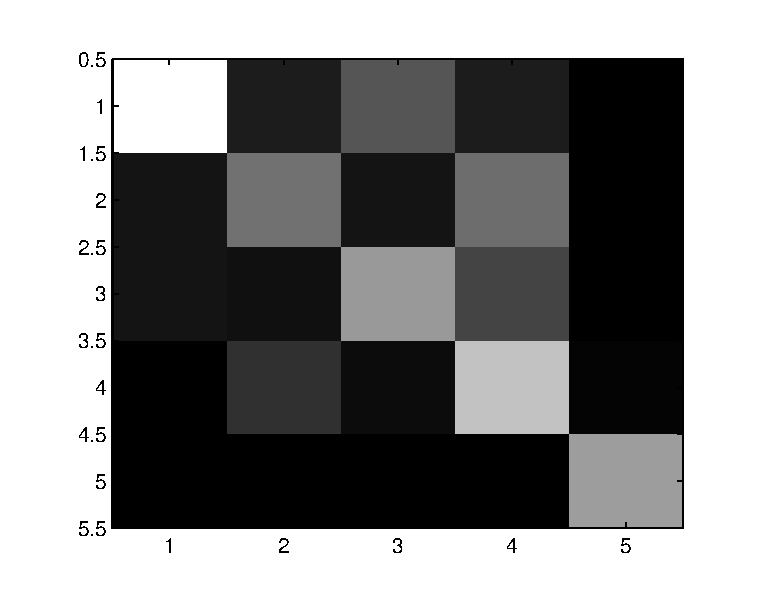
\includegraphics[width=50mm]{confusion_Ppat.eps}

	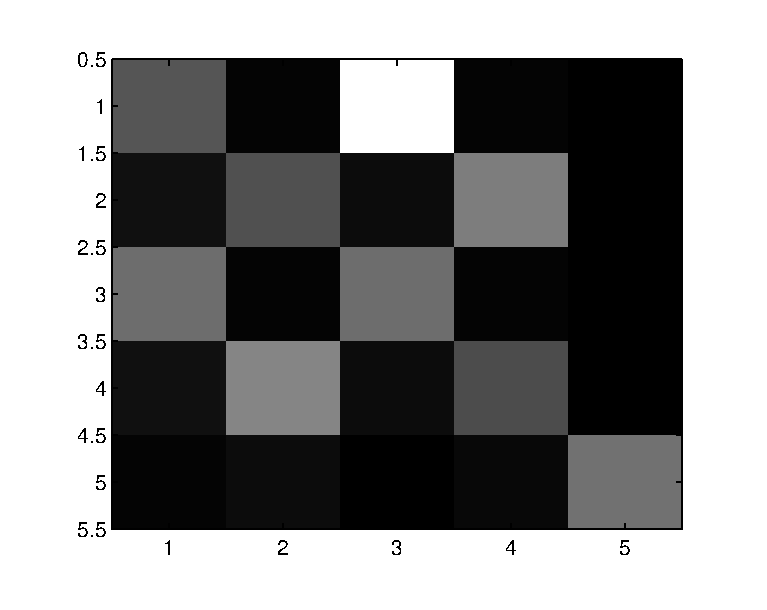
\includegraphics[width=50mm]{confusion_freq.eps}
	\end{multicols}
	\caption{Слева: confusion matrix для классификации по P-Паттернам, справа: по частотам и средним продолжительностям.}
\end{figure}
\end{frame}

\begin{frame}
  \frametitle{Общие паттерны}
  Параметры каждого паттерна подгоняются под конкретное наблюдаемое поведение. 
  \begin{itemize}
  \item Вариант I. Ищем паттерны, найденные у одного животного в поведении других. Подсчет правдоподобия. Ослабить параметры.
  \item Вариант II. В процедуре конструирования паттренов рассматривать животных не по отдельности, а вместе. 
  \end{itemize}
\end{frame}

\begin{frame}
  \frametitle{Характерные паттерны}
   \begin{itemize}
  \item 2 группы: контроль(12 особей), гиппокампальная(12 особей).
  \item Всего в 24-ех файлах найдено 1150 P"=Паттернов. 
  \item Берем только P"=Паттерны, содержащие 5 и больше событий.
  \item Для каждого такого P"=Паттерна говорим, что он присутствует в 
       поведении особи $i,\;(i=1,\dots, 24)$, если в этом поведении найдено больше, чем $N_{min}=3$ экземпляра паттерна. 
  \item P-Паттерн характерен для группы, если он встречается у многих особей из данной группы и редко встречается 
у особей из других групп.
  
   \end{itemize}
\end{frame}

\begin{frame}
  \frametitle{Характерные P-Паттерны}
\begin{figure}[h]
\noindent\centering{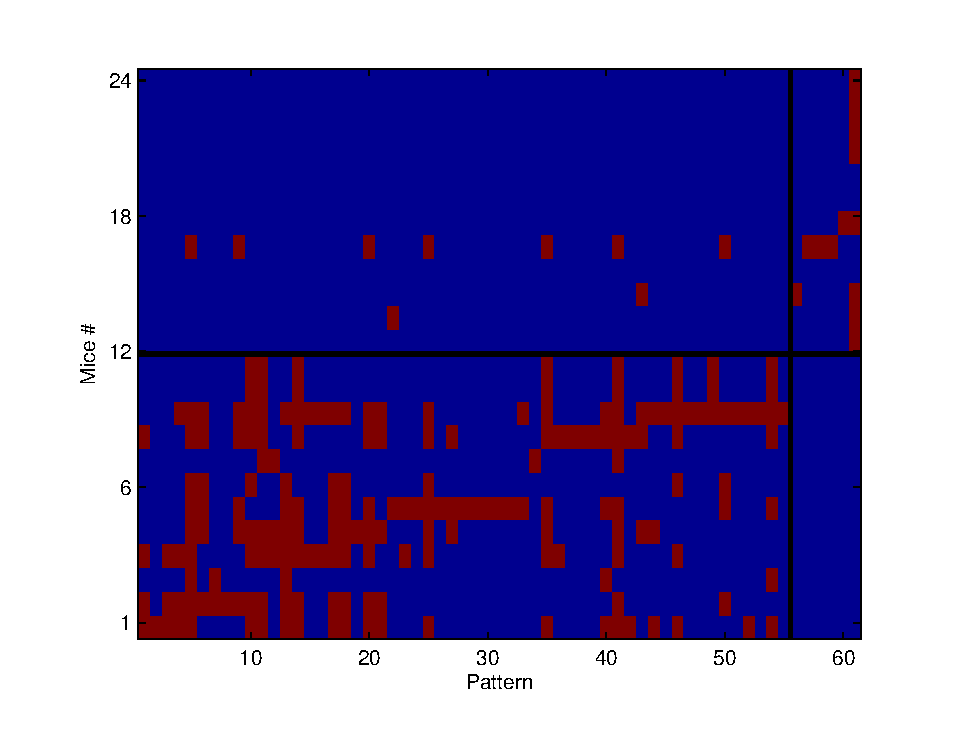
\includegraphics[width=93mm]{char_pat.eps}}

\end{figure}
\end{frame}

\begin{frame}
  \frametitle{Характерные T-Паттерны}
\begin{figure}[h]
\noindent\centering{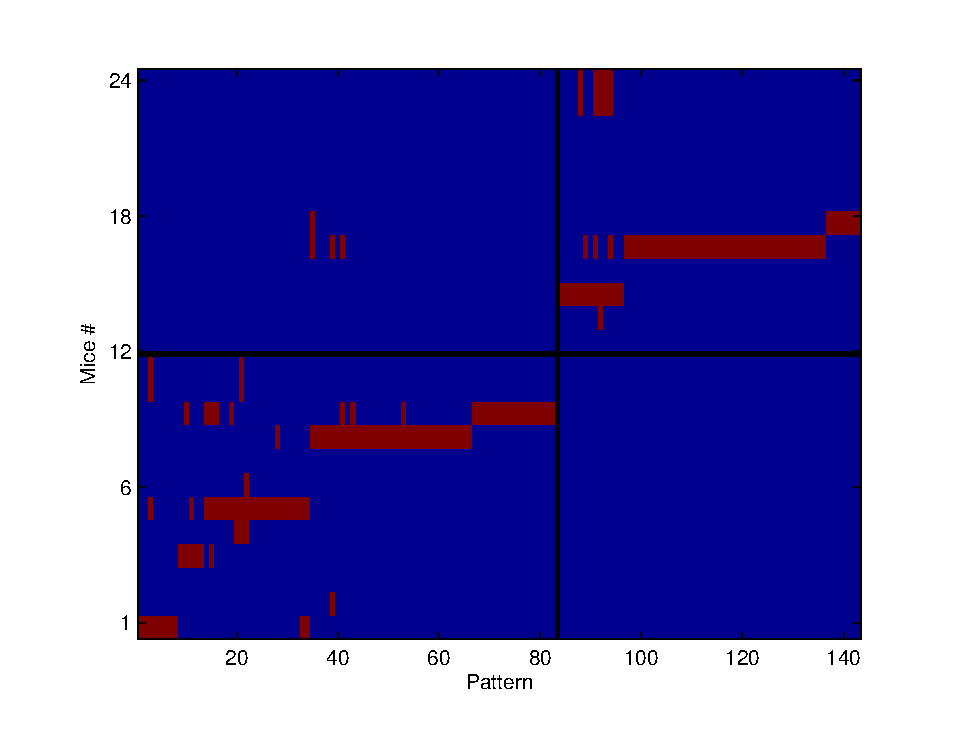
\includegraphics[width=93mm]{char_tpat.eps}}
\end{figure}
\end{frame}

\begin{frame}
  \frametitle{Один из характерных P-Паттернов контрольной группы}
 Вычесывание задними конечностями $[22.9;\; 7.9]$
 Вылизывание ладоней $[1.1;\; 2.7]$
 Быстрое умывание носа $[0.4;\; 0.5]$
 Умывание головы с ушами $[ 3.2;\; 7.9 ]$
 Умывание носа $[ 17.0;\; 7.9 ]$
 Вылизывание задних конечностей
 \\ ~\\


 Найден у 9 из 12 особей контрольной группы и ни разу не найден в гиппокампальной группе.
\end{frame}

\begin{frame}
  \frametitle{Отклик на P-Паттерн в контрольной группе}
\begin{figure}[h]
\noindent\centering{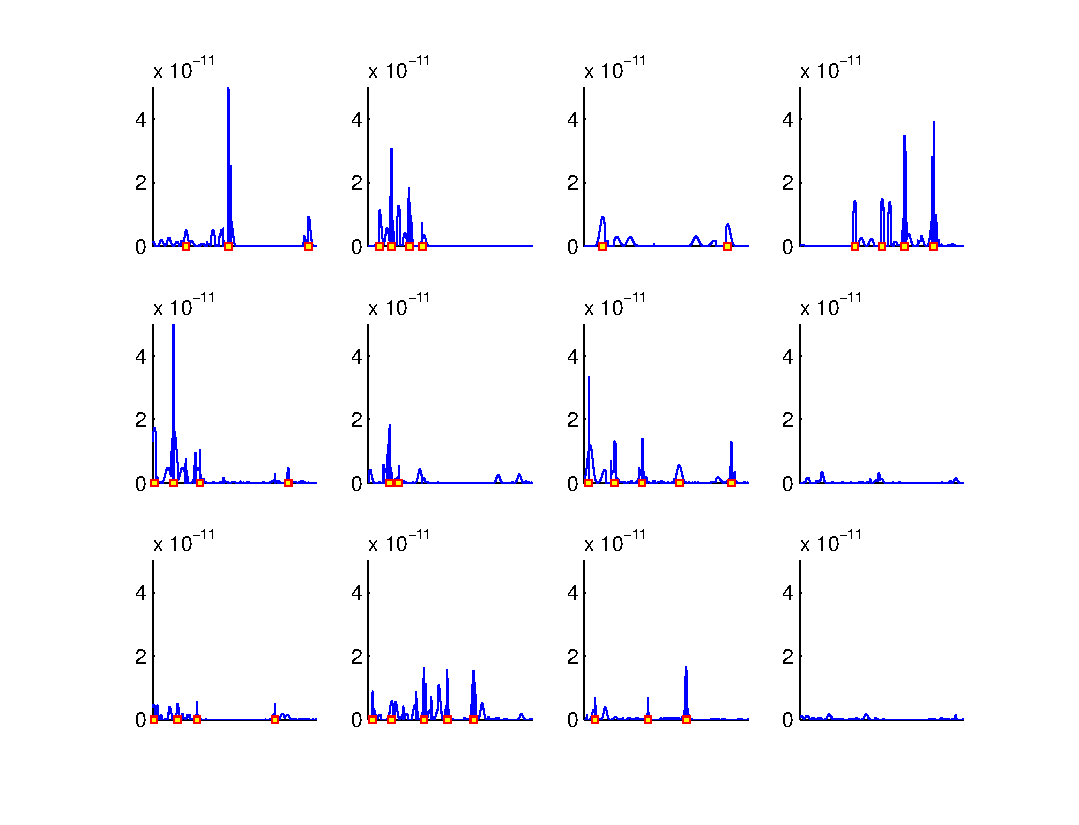
\includegraphics[width=93mm]{patLH_contr.eps}}
\end{figure}
\end{frame}

\begin{frame}
  \frametitle{Отклик на P-Паттерн в гиппокампальной группе}
\begin{figure}[h]
\noindent\centering{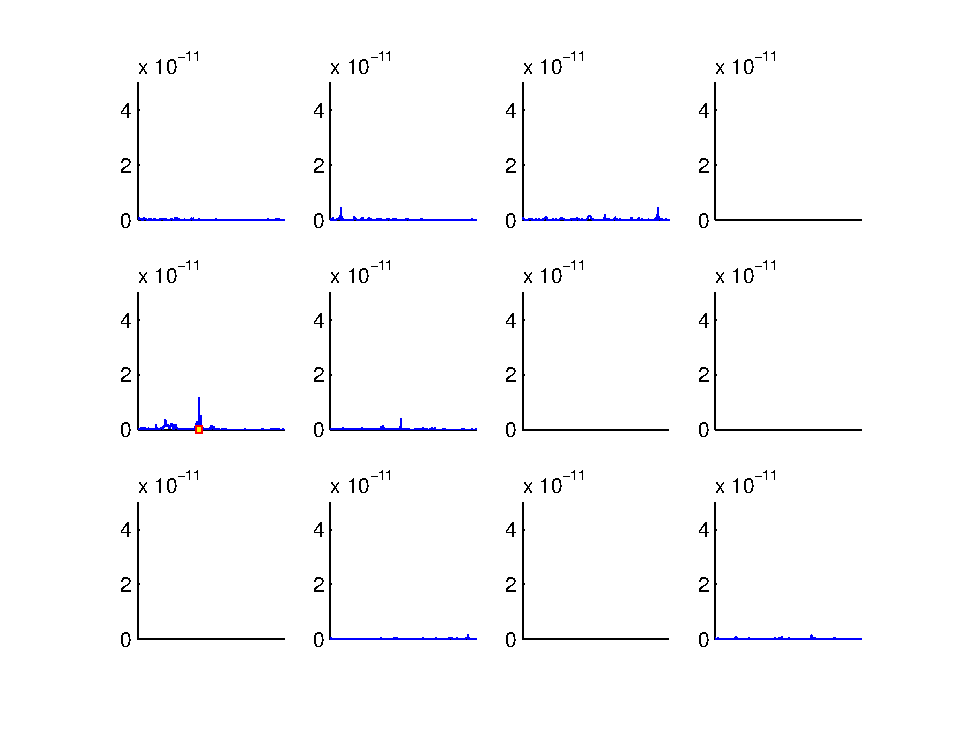
\includegraphics[width=93mm]{patLH_hip.eps}}
\end{figure}
\end{frame}


\section{Заключение}



\begin{frame}
  \frametitle{Выводы}
  \begin{itemize}
   \item Предложенный метод расширяет существующий подход
	  к поиску паттернов.
   \item Устойчивость к шуму.
   \item Достигнуто ускорение параллельной версии на GPU в 40 раз.
   \item Качество классификации на экспериментальных данных $\sim$ 92\%.
   \item Предложенный метод применим не только для анализа поведения животных(структура ДНК, спайковая активность нейронов, рынки, новостные тренды).

\item[$-$] Сложности на очень маленьких объемах данных.
\item[$-$] Долгое время работы на очень больших объемах данных.
  \end{itemize}
\end{frame}


\end{document}

